\selectlanguage{english}%

\chapter{Introduction}


\section{Standard model and Quantum Chromodynamics}

The Standard Model of particle physics is a theory concerning the
electromagnetic, weak, and strong nuclear interactions, which explains
how the basic building blocks of matter interact. The Standard Model
includes members of several classes of elementary particles: 12 elementary
particles of spin 1/2 known as fermions, 4 gauge bosons of spin 1
who carry the force of fundamental interactions and Higgs boson of
spin 0 which interacts with elementary particles and gives them mass.
The 12 fermions includes 6 quarks (up (\emph{u}), down (\emph{d}),
strange (\emph{s}), charm (\emph{c}), top (\emph{t}), bottom (\emph{b})),
and 6 leptons (electron (\emph{e}), muon ($\mu$), tau ($\tau$) and
the corresponding neutrinos). The 4 gauge bosons are gluon (\emph{g}),
photon ($\gamma$), \emph{W} and \emph{Z} bosons, which are classified
by the fundamental force they carry. Gluons mediate the strong interactions
between color charged particles (quarks). Gluons also carry color
charge, so they can also interact with themselves. The strong interaction
are described by the theory of quantum chromodynamics. The electric
charged particles interact through the electromagnetic force mediated
by Photons which is well-described by the theory of quantum electrodynamics.
The weak force is carried by \emph{W} and \emph{Z} bosons. They are
grouped with photons, as collectively mediation the electroweak interaction.
Figure \ref{fig:SM} shows the particles generations and interactions
between them. Fermions interact with each other through the fundamental
force carried by gauge bosons and form the matter world. On 14 March
2013, the Higgs boson was tentatively confirmed to exist. 

\begin{figure}
\begin{centering}
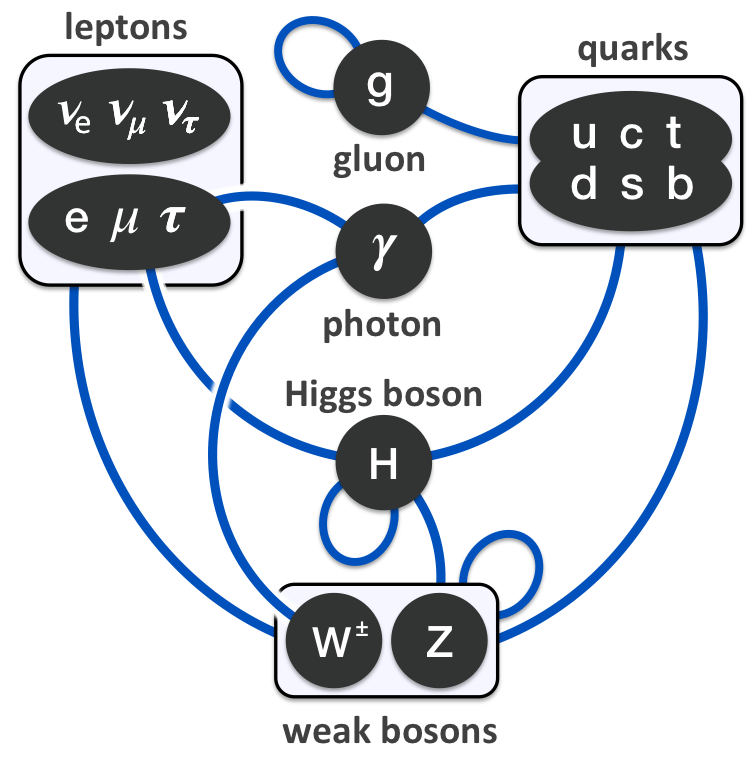
\includegraphics[width=0.8\textwidth]{fig/1.Introduction/Standard_Model}
\par\end{centering}

\protect\caption{Summary of interactions between particles described by the Standard
Model.}


\label{fig:SM}
\end{figure}



\subsection{Quantum Chromodynamics (QCD)}

In the 1950s, a large number of strongly interacting particles (hadrons)
were discovered in particle physics experiments. To understand and
explained the spectrum of these particles, in 1963, Gell-Mann and
Zweig proposed a model in terms of elementary constituents called
\emph{quarks. }The hadrons could be sorted into groups having similar
quantum properties by the existence of three flavors of quarks inside
hadrons. Mesons were expected to be quark-antiquark bound states,
while baryons were interpreted as bound states of three quarks. To
explain the electric charges and other quantum numbers of hadrons,
Gell-Mann and Zweig assumed three species of quarks, up (\emph{u}),
down (\emph{d}) and strange (\emph{s}). With the discovery of more
hadrons, the quarks family were extended of three more species: charm
(\emph{c}), bottom (\emph{b}) and top (\emph{t}). To make baryons
with integer charges, the quarks were assigned fractional electric
charge: +2/3 for \emph{u}, \emph{c, t, }and -1/3 for \emph{d}, \emph{s},
\emph{b. }And all quarks were assumed to be spin-1/2. The quark model
had great success in predicting new hadronic states, but some hadrons
composed with three identical quarks with parallel spin, such as $\varDelta^{++}$(\emph{uuu}),
are forbidden by the Pauli exclusion principle. To solve this problem,
Han and Nambu, Greenberg, and Gell-Mann introduced an additional SU(3)
gauge degree of freedom of quarks called \emph{color }and an octet
of vector gauge bosons called gluons to carry the interaction between
quarks. In 1972, Gell-Man and Fritzsch introduced the Quantum Chromodynamics
(QCD) to describe the strong interaction between the colored quarks
and gluons.

The QCD Lagrangian can be written as:

\begin{equation}
\mathcal{L_{{\rm QCD}}}=-\frac{1}{4}F_{a}^{\mu\nu}F_{\mu\nu}^{a}+\underset{f}{\sum}\bar{q_{f}}^{i}i\gamma^{\mu}(D_{\mu})_{ij}q_{f}^{j}-\underset{f}{\sum}m_{f}\bar{q}_{f}^{i}q_{f}^{i}\label{eq:LQCD}
\end{equation}
\begin{equation}
F_{a}^{\mu\nu}=\partial^{\mu}G_{a}^{\nu}-\partial^{\nu}G_{a}^{\mu}+g_{s}f^{abc}G_{b}^{\mu}G_{c}^{\nu}\label{eq:fieldStr}
\end{equation}
\begin{equation}
D^{\mu}=\partial^{\mu}-ig_{s}\frac{\lambda^{a}}{2}G_{a}^{\mu}\label{eq:cd}
\end{equation}
where $g_{s}$ is the QCD coupling constant, and the $f^{abc}$ are
the structure constants of the $SU(3)_{C}$ algebra. $q_{f}^{i}$
defines a quark field with color \emph{i} and flavor \emph{f }, while
$\gamma^{\mu}$ are the Dirac matrices. $F_{a}^{\mu\nu}$ are the
field strengths tensor which were introduced to describe the self
interaction of the gluon fields. $D^{\mu}$ are the covariant derivative
with the Gell-Mann matrices $\lambda^{a}$ and the Yang-Mills (gluon)
fields $G_{\mu}^{a}(x)$ where $a=$1, 2, ..., 8.


\subsection{Running coupling}

The effective QCD coupling constant $\alpha_{s}(\mu)$ can be written
as:

\begin{equation}
\alpha_{s}(\mu)\equiv\frac{g_{s}^{2}(\mu)}{4\pi}\approx\frac{4\pi}{\beta_{0}\ln(\mu^{2}/\Lambda_{QCD}^{2})}
\end{equation}
Where $\beta_{0}$ is a constant larger than 0 which dependence on
the number of quarks with mass less than the energy scale $\mu$.
The coupling $\alpha_{s}(\mu)$ shows a dependence on the renormalization
scale. Figure \ref{fig:QCD_as} shows the measurements of $\alpha_{s}$
as a function of the energy scale \emph{Q. }The world average result
of $\alpha_{s}(M_{z}^{2})=0.1179\pm0.0008$ \cite{PhysRevD.86.010001}
and the QCD scale is $\Lambda_{QCD}$\textasciitilde{}200 MeV. With
decreasing interaction distance and increasing momentum transfer,
the coupling constant decreases, the interaction between quarks and
gluons goes weaker. This is the major feature of QCD: asymptotic freedom.
While the energy scale $\mu\ll\Lambda_{QCD}$ (short distance and
high momentum transfer), QCD can be described with perturbative method
(perturbative QCD). On the other hand, pQCD breaks down when the $\mu\sim\Lambda_{QCD}$
where QCD becomes strongly coupled. People introduced Lattice QCD
to calculated QCD in this case. 

\begin{figure}
\begin{centering}
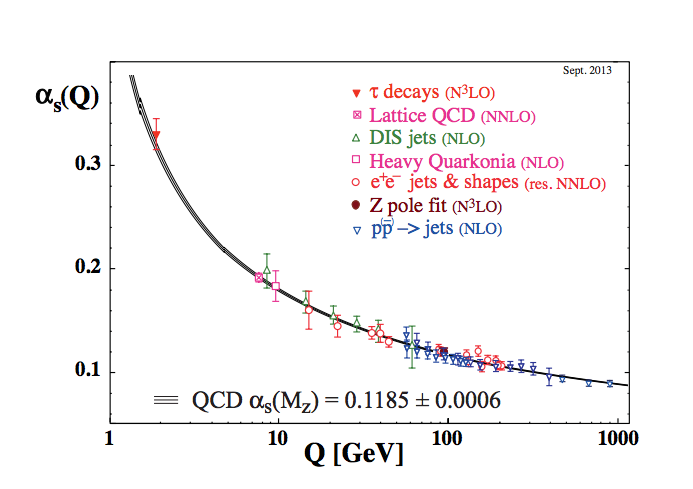
\includegraphics[width=0.8\textwidth]{fig/1.Introduction/QCD_as}
\par\end{centering}

\protect\caption{Summary of measurements of $\alpha_{s}$ as a function of the energy
scale\emph{ Q}. Figure is taken from \cite{PhysRevD.86.010001}.}


\label{fig:QCD_as}
\end{figure}



\subsection{Chiral symmetry}

We consider the Lagrangian of two flavors massless fermions, and the
results will be directly applicable to massless QCD. The Lagrangian
is given by:

\begin{equation}
\mathcal{L}=i\bar{\psi_{j}}\gamma_{\mu}\partial^{\mu}\psi_{j}\label{eq:L_massless}
\end{equation}
where the index \emph{j }presents the two different flavors (\emph{u},
\emph{d}). Consider two transformation :
\begin{enumerate}
\item vector transformation $\Lambda_{V}$ :
\begin{equation}
\Lambda_{V}:\;\psi\rightarrow e^{-i\frac{\vec{\tau}}{2}\vec{\Theta}}\psi\simeq(1-i\frac{\vec{\tau}}{2}\vec{\Theta})\psi
\end{equation}
and its conjugate form:
\begin{equation}
\Lambda_{V}:\;\bar{\psi}\rightarrow e^{+i\frac{\vec{\tau}}{2}\vec{\Theta}}\bar{\psi}\simeq(1+i\frac{\vec{\tau}}{2}\vec{\Theta})\bar{\psi}
\end{equation}
where $\vec{\tau}$ is the Pauli-spin-matrices and $\vec{\Theta}$
are the rotation angle. $\psi$ is the Dirac iso-spinor for fermions,
$\psi=(\psi_{u},\psi_{d})$. Clearly the Lagrangian is invariant under
$\Lambda_{V}$ and the associated conserved current is 
\begin{equation}
V_{\mu}^{a}=\bar{\psi}\gamma_{\mu}\frac{\tau^{a}}{2}\psi
\end{equation}

\item axial transformation $\Lambda_{A}$
\begin{align}
\Lambda_{A}:\;\psi & \rightarrow e^{-i\gamma_{5}\frac{\vec{\tau}}{2}\vec{\Theta}}\psi\simeq(1-i\gamma_{5}\frac{\vec{\tau}}{2}\vec{\Theta})\psi\\
\bar{\psi} & \rightarrow e^{-i\gamma_{5}\frac{\vec{\tau}}{2}\vec{\Theta}}\bar{\psi}\simeq(1-i\gamma_{5}\frac{\vec{\tau}}{2}\vec{\Theta})\bar{\psi}
\end{align}
The Lagrangian transforms as following :
\begin{equation}
i\bar{\psi}\gamma^{\mu}\partial_{\mu}\psi\rightarrow i\bar{\psi}\gamma^{\mu}\partial_{\mu}\psi-i\vec{\Theta}(\bar{\psi}i\partial_{\mu}\gamma^{\mu}\gamma_{5}\frac{\vec{\tau}}{2}\psi+\bar{\psi}\gamma_{5}\frac{\vec{\tau}}{2}i\partial_{\mu}\gamma^{\mu}\psi)
\end{equation}
since $\gamma_{5}$ anti-commutes with $\gamma_{\mu}$, the last term
vanishes. Therefore the Lagrangian is also invariant under $\Lambda_{A}$
with the conserved 'axial-vector' current: 
\begin{equation}
A_{\mu}^{a}=\bar{\psi}\gamma_{\mu}\gamma_{5}\frac{\tau^{a}}{2}\psi
\end{equation}

\end{enumerate}
So, the Lagrangian of massless QCD is invariant under the vector and
axial transformations. This symmetry is called \emph{chiral symmetry}.
If we introduce a mass term in the Lagrangian.
\begin{equation}
\delta\mathcal{L}=-m(\bar{\psi}\psi)
\end{equation}
It can easily prove the $\delta\mathcal{L}$ is invariant under the
vector transformations, but the axial transformations symmetry is
broken. In case of QCD, the mass of the light quarks are very small
(about 5\textasciitilde{}10 MeV) comparing to the QCD energy scale
which is about 200 MeV. Therefore, the $\Lambda_{A}$ should be an
approximate symmetry. And the slight symmetry breaking due to the
quark masses is called Partial Conserved Axial Current hypothesis
(PCAC).


\subsection{Spontaneous breaking of chiral symmetry}

The conservation of chiral symmetry leads to a direct deduction that
the chiral partner which can be rotated into each other by the operation
$\Lambda_{A}$ should have the same masses, since they should have
the same Eigenvalues. However, in the real world, this is clearly
not true, since the chiral partner $\rho$ and $a_{1}$ have quite
difference masses ($m_{\rho}=770$ MeV and $m_{a_{1}}=1260$ MeV)
which should be degenerate if the chiral symmetry is conserved. In
additional, this can not be explained by the slight symmetry breaking
due to the finite current quark masses, which should lead to a mass
difference much smaller than the particle mass. However, the mass
difference between $\rho$ and $a_{1}$ is of the same order as $\rho$
mass. On the other hand, let us consider the weak decay of pion which
is controlled by the matrix element of the axial current between vacuum
and pion 
\begin{equation}
\left\langle 0|A_{\mu}^{a}(x)|\pi^{b}(q)\right\rangle =-if_{\pi}q_{\mu}\delta^{ab}e^{-iq\cdot x}\label{eq:pi_wd}
\end{equation}
and $f_{\pi}$ is a constant \textasciitilde{} 93 MeV which measures
the strength of the symmetry breaking. If we take the divergence of
eq. \ref{eq:pi_wd}
\begin{equation}
\left\langle 0|\partial^{\mu}A_{\mu}^{a}(x)|\pi^{b}(q)\right\rangle =-if_{\pi}q_{\mu}q^{\mu}\delta^{ab}e^{-iq\cdot x}=-f_{\pi}m_{\pi}^{2}\delta^{ab}e^{-iq\cdot x}
\end{equation}
, comparing to the hadronic scales, the pion mass is vanishing, thus
the axial current is approximately conserved which supports for the
conservation of chiral symmetry. 

To solve the contradiction discussed above, the spontaneous breakdown
of chiral symmetry was introduced. The breaking of symmetry has two
conditions: explicit breaking, which is due to the explicit asymmetry
in the Lagrangian, i.e. the finite mass of quarks in QCD; spontaneous
breaking, which means the symmetry is not realized in the ground state.
We considering effective potentials shown in fig \ref{fig:sbsc}.
Panel (a) shows a potential with ground state just in the middle.
The ground state plus potential are invariant under rotations. In
panel (b), any points in the valley can be the ground state. If we
chosen as one direction as the ground state, the axial rotation symmetry
is obviously spontaneously broken, since the Lagrangian is invariant
but the vacuum is not. 

The QCD vacuum of quark-antiquark condensate $\left\langle 0\left|\bar{q}q\right|0\right\rangle $
can be related to $f_{\pi}$ by the Gell-Mann-Oakes-Renner relation
(GOR):
\begin{equation}
m_{\pi}^{2}f_{\pi}^{2}=-2\bar{m}\left\langle 0\left|\bar{q}q\right|0\right\rangle 
\end{equation}
where $\bar{m}$ is the average mass of up and down quarks. If taking
$\bar{m}$ = 6 MeV, then the vacuum of quark antiquark condensate
is about $\left\langle 0\left|\bar{q}q\right|0\right\rangle \approx(-250MeV)^{3}$
per light flavor. The non-zero vacuum spontaneously breaks the chiral
symmetry of QCD. Since chiral symmetry is a global symmetry, its spontaneous
breaking must be accompanied by (almost) massless Goldstone bosons.
In case of two light quark flavors, the three charge states of the
pion servers as the Goldstone bosons, with a mass (about 140 MeV)
which is much smaller comparing to all the other hadrons. The assumption
of spontaneously broken axial-vector symmetry also explains the large
mass splitting between $\rho$ and $a_{1}$ meson. Theory calculations
predict that $m_{a_{1}}=\sqrt{2}m_{\rho}$ \cite{PhysRevLett.18.507}.

\begin{figure}
\begin{centering}
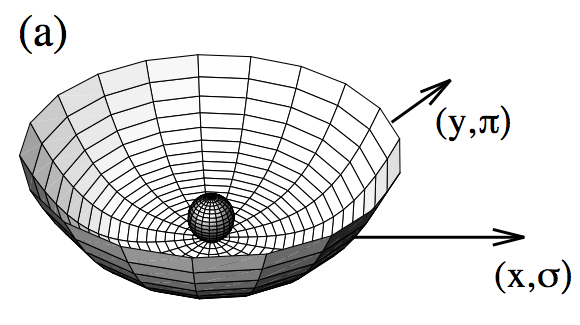
\includegraphics[width=0.45\textwidth,height=0.16\paperheight]{fig/1.Introduction/nosbcs}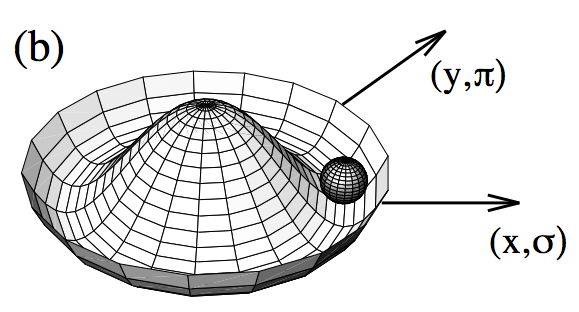
\includegraphics[width=0.45\textwidth,height=0.16\paperheight]{fig/1.Introduction/sbcs}
\par\end{centering}

\protect\caption{(a) No spontaneous breaking of symmetry. (b) Spontaneous breaking
of symmetry.}


\label{fig:sbsc}
\end{figure}



\subsection{Deconfinement and QGP}

Another important feature of QCD is confinement which lead to the
absence of direct observation of isolated quarks and gluons in the
experiment. The confinement is because gluons who carry the force
have color charge and thus can interact with itself. Due to the property
of the running QCD coupling constant $\alpha_{s}$, when two quarks
are separated from each other, the force between them grows stronger
as the distance increasing. When the energy is enough, a new quark/anti-quark
pair is created from the vacuum. As result of this, the quarks and
gluons are confined inside hadrons, and when quarks is created in
high energy experiment, instead of seeing the individual quarks, only
cluster of color neutral hadrons are observed. This process is called
hadronization. On the other hand, when the system is at extreme temperature
or high energy density, such like the universe in a few microsecond
after the ``Big Bang'', due to the asymptotic freedom, the interaction
between partons (quarks/anti-quarks and gluons) is very weak and the
partons can travel over larger distances of the size of a nucleon
(\textasciitilde{}1 fm). The quarks and gluons are deconfined and
form a thermalized state known as Quark-Gluon Plasma (QGP) \cite{PhysRevLett.34.1353}.

The lattice QCD calculations expect a phase transition from the hadronic
phase into the QGP phase. The\emph{ Polyakov loop operator,
\begin{equation}
L=\frac{1}{3}{\rm tr}\left(\mathcal{P}e^{ig\intop_{0}^{\beta}A_{4}(x,\tau)d\tau}\right)
\end{equation}
}is believed as a observable for the phase transition. Figure \ref{fig:ptxs}
left shows the Polyakov loop operator expectation value $\left\langle L\right\rangle $
and its temperature derivative as a function of the lattice coupling
$\beta=6/g^{2}$. At small temperature, a vanishing thermal expectation
value $\left\langle L\right\rangle $ of Polyakov loop operator indicates
infinite energy for a free quark, or in another word, quark is confined.
At high temperature, $\left\langle L\right\rangle $ increase rapidly
to a nonzero value, its derivative shows a sharp peak at a critical
coupling $\beta_{cr}$. This indicates that quark is deconfined at
the corresponding critical temperature $T_{cr}$. Figure \ref{fig:Phase_diagram}
shows the phase diagram of strongly interacting matter in temperature
vs. baryon chemical potential plane ($T$, $\mu_{B}$). The lattice
QCD calculations tell us the phase transition alone the temperature
axis ($\mu_{B}$ = 0), with a crossover transition from hadron resonance
gas to a QGP phase at a temperature about 154 MeV. On other hand,
QCD based models indicate that the crossover transition ends at a
critical point at high $\mu_{B}$ and becomes first order transition
\cite{PhysRevD.78.074507,PhysRevC.79.015202}. However, the locations
of the phase boundary and the critical point in this framework depend
on model assumptions. One of the main aim of high-energy heavy-ion
collision experiments is to explore the QCD phase diagram, to locate
the position of critical point, and to determine the QCD phase boundary.

\begin{figure}
\begin{centering}
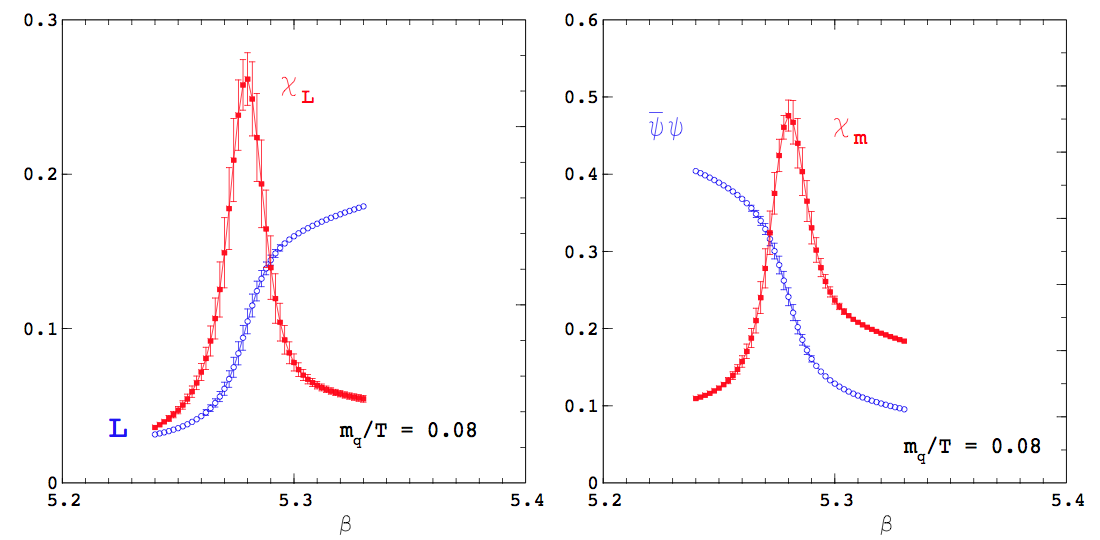
\includegraphics[width=0.9\textwidth]{fig/1.Introduction/phase_transition_xsymmtry}
\par\end{centering}

\protect\caption{Left panel: the expectation value of Polyakov loop $\left\langle L\right\rangle $
and its temperature derivative (Polyakov loop susceptibility $\chi_{L}$)
as a function of the lattice coupling $\beta=6/g^{2}$ which is related
to the temperature $T$ (larger $\beta$ correspond to larger $T$).
Right panel: the chiral condensate (the scalar quark density) $\left\langle \bar{\psi}\psi\right\rangle $
and the negative of its temperature derivative (chiral susceptibility
$\chi_{m}$) as a function of temperature. \cite{PhysRevD.50.6954,Heinz:fk}}


\label{fig:ptxs}
\end{figure}


\begin{figure}
\begin{centering}
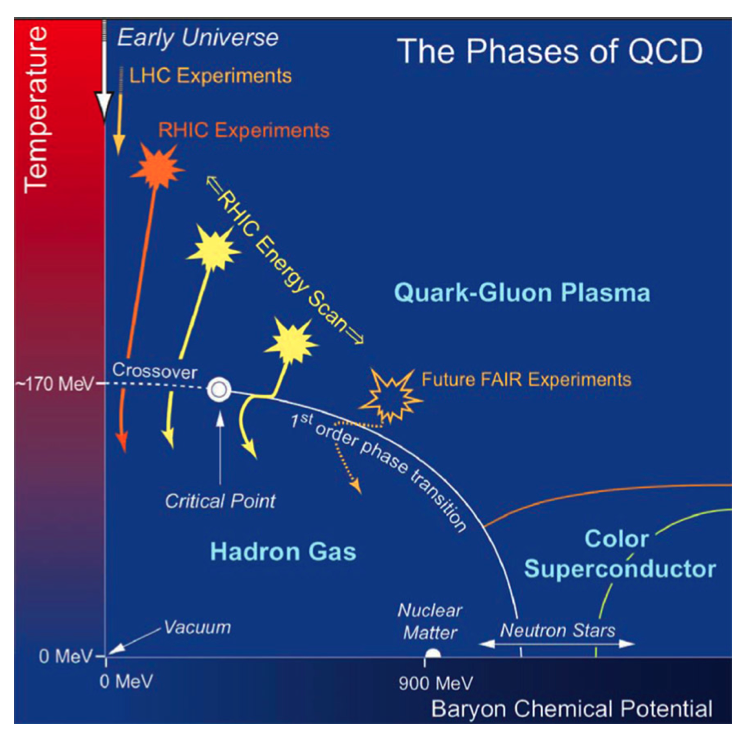
\includegraphics[width=0.8\textwidth]{fig/1.Introduction/QCD_Phase_diagram}
\par\end{centering}

\protect\caption{A conjectured QCD phase diagram with boundaries that define various
states of QCD matter. \cite{STAR-Collaboration:2014qf}}


\label{fig:Phase_diagram}
\end{figure}



\subsection{Restoration of the chiral symmetry}

Another feature of the hot and density strongly interacting matter
is the restoration of the chiral symmetry. Considering the chiral
quark-antiquark condensate $\left\langle \bar{\psi}\psi\right\rangle $,
figure \ref{fig:ptxs} right panel shows $\left\langle \bar{\psi}\psi\right\rangle $
as and its temperature derivative as a function of the lattice coupling
$\beta=6/g^{2}$ (a value corresponding to the temperature). The nonvanishing
chiral condensate at T = 0 spontaneously breaks the chiral symmetry
and generates a dynamic mass of order 300 MeV for up and down quarks.
With the temperature increasing, the dynamically generated mass melts
away at $T_{cr}$, and the quarks mass become vanishing again above
$T_{cr}$, or in another word, the approximate chiral symmetry is
restored. Numerical computations of the lattice-discretized path integral
for QCD at finite temperature predict chiral symmetry restoration
to happen at a critical temperature of $T_{c}\approx160-190$ MeV,
corresponding to an energy density of about $\varepsilon_{c}\approx1{\rm GeV/fm^{3}}$
\cite{PhysRevD.74.054507,Aoki200646}. If considering the quark component
in real world (two light quarks $u$ and $d$, and a much heavier
strange quarks), this transition is more likely a rapid cross-over.

Chiral symmetry restoration can be characterized by the rapid decrease
of the $\bar{q}q$ condensate, while in experiment, the key manifestations
are its consequences for the hadron spectrum. Chiral partners must
degenerate which lead to a massive medium modifications of hadronic
spectral functions as the transition is approached. The $\rho$ meson
is a unique tool for characterizing the chiral properties of hot and
density medium, since its life time is much short (\textasciitilde{}1.3
fm) than the medium (\textasciitilde{}10 fm). Its spectral functions
is expected to be significant modified (comparing to other light mesons)
during the interaction with medium. There are two main scenarios on
the in medium modification of the $\rho$ meson. Brown and Rho suggests
that the $\rho$-meson mass should drop to almost zero as a consequence
of chiral symmetry restoration \cite{PhysRevLett.66.2720,Brown1996333}.
Subsequently, more medium modifications of the $\rho$ meson were
investigated based on its rescattering on constituents of a hadronic
medium, \cite{R.-Rapp:2000uq,Cassing199965,Gale:2003qv,Alam2000159}.
These calculation based on hadronic many-body interactions predict
a strong broadening of the $\rho$ spectral function, which when when
extrapolated to the putative phase transition temperature, leading
to a complete “melting” of the resonance structure. Figure \ref{fig:Meson_Medium}
right panel shows the scenarios for the effects of chiral symmetry
restoration on the in-medium vector- and axial-vector spectral functions. 

\begin{figure}
\begin{centering}
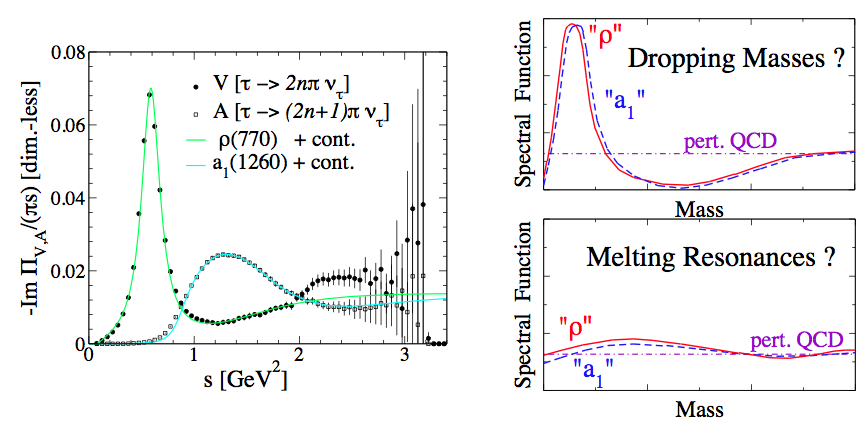
\includegraphics[width=0.8\textwidth]{fig/1.Introduction/Vector_Mason_chiral}
\par\end{centering}

\protect\caption{Left panel: vector and axial-vector spectral functions as measured
in hadronic $\tau$ decay \cite{Barate-et-al.:1998fk}. Right panel:
scenarios for the effects of chiral symmetry restoration on the in-medium
vector- and axial-vector spectral functions. Figure is taken from
\cite{R.-Rapp:hl}.}


\label{fig:Meson_Medium}
\end{figure}



\section{Dilepton production in high energy heavy ion collisions}

The heavy ion collision is believed to be the best way to study properties
of QCD matter in laboratory, since increasing the mass number of the
incident particles is more efficient than increasing beam energy.
During the past 20 years, world wide effort has been dedicated in
this region. Several large-scale experiments have been conducted.
Relativistic heavy ion collider (RHIC) built in Brookhaven National
Laboratory is the first accelerator-collider dedicated to heavy ion
collisions. During the first few years of its operation, plenty measurements
support the existence of a new matter form: a strongly coupling Quark
Gluon Plasma (sQGP). Currently the physics program at RHIC was changing
to studying the property of strongly interacting matter created in
high energy heavy ion collisions and searching for phase boundary
and critical point of the QGP phase diagram. At CERN, the Large Hadron
Collider (LHC) also contributes in the heavy ion collisions program.
It is pushing the colliding energy up to 5.5 TeV, where the energy
density and temperature is much higher than the requirement of QGP
formation.

Probes explored in experiments are mostly hadrons which have been
used to demonstrate the formation of a strongly-coupled Quark Gluon
Plasma (sQGP) in high energy heavy ion collision at RHIC and LHC.
Dileptons as an electromagnetic probe, escape the interacting system
without suffering further strong interactions after production. In
additional, dilepton can be produced on the various stages of entire
system evolution. They are therefore expected to be an outstanding
probes to study the property of the medium created in high energy
heavy ion collisions. 

Traditionally, due to different physics of interest, the dilepton
kinematic phase space is divided into the Low Mass Region - LMR ($M_{ll}<M_{\phi}$),
the Intermediate Mass Region - IMR ($M_{\phi}<M_{ll}<M_{J/\psi}$)
and the High Mass Region - HMR ($M_{ll}>M_{J/\psi}$). 

At the initial stage of the system, the initial hard pQCD process
Drell-Yan production ($q\bar{q}\rightarrow l^{+}l^{-}$) can produce
high mass dilepton and is thus expected to dominate in the HMR. Moreover,
direct photons form the initial hard scattering can allow for bremsstrahlung
emission of soft virtual photons which convert into low mass and high
transverse momentum ($p_{T}$) dielectrons (``internal conversion'').
These dilepton, in principle, can be calculated within the pQCD frame.

The system is expected to quickly reach the partonic sQGP phase where
dileptons can be produced in thermal radiation via multiple parton-parton
scattering. Theoretical calculations suggest that at top RHIC energy,
QGP thermal dilepton production will become dominant in the IMR while
thermal dileptons with higher masses originate from earlier stages
\cite{PhysRevC.63.054907}. This indicates that investigating the
thermal dilepton production in $M_{ll}$ \& $p_{T}$ allows for probing
the medium properties at different stages of the space-time evolution.
Measuring thermal dilepton collective flow and polarization can reveal
information about the degrees of freedom of deconfinement and equilibrium
of the strongly interacting matter created in heavy ion collisions\cite{Deng2011581,PhysRevC.75.054909,Shuryak:qy}.
Thermal radiation can produce real photons accompanied by low mass
and high $p_{T}$ dileptons. Study of these dileptons compared to
that from initial hard scattering, one can learn the direct real photon
production from the thermal QGP medium. 

The system expands, cools and enters into the hadronic phase. Dileptons
emitted from the hadronic medium are governed by the coupling of vector
mesons ($\rho,\:\omega,\:\phi$ etc) to the medium via hadron-hadron
interaction and are expected to dominate LMR production \cite{R.-Rapp:2000uq}.
Their mass spectra are determined by the chiral properties of QCD
which is spontaneously broken in vacuum. Theoretical calculations
suggest that the vector meson spectral functions will be modified
in the hot and dense hadronic medium, which may be connected to the
restoration of chiral symmetry. Among them, the $\rho$ meson is expected
to most modified, due to its short life time \textasciitilde{} 1.3
fm comparing to the lift time of hadronic medium (\textasciitilde{}
10 fm) \cite{Pisarski1982155}. Two scenarios have been proposed for
the change of vector meson spectral functions when chiral symmetry
is restored: a shift of the pole mass \cite{Brown1996333} and a broadening
of the mass spectral function \cite{Rapp:1999kx}. Measurements of
dielectron continuum in the low mass region will shed light on the
vector meson production mechanism, and hence the medium chiral properties
in heavy ion collisions.

Finally, when all particles decouple from the system long-lived $\pi^{0}$,
$\eta$, $D\bar{D}$ etc. can decay into lepton pairs and be measured
by the detector system. Their contributions can be calculated based
on the measured or predicted invariant yields of parent mesons. Usually,
their contributions are called hadronic decay cocktail.


\section{Previous experiments and measurements}

Dilepton measurements in heavy ion collisions have been pursued for
decades in different collision system from low to relativistic energies\cite{PhysRevLett.75.1272}.
In this section, I will make a brief review of several important experiment
measurements from SPS and RHIC.


\subsection{CERES/NA45}

NA45 collaboration a fixed-target heavy ion collisions experiment
at the CERN Super Proton Synchrotron (SPS). It is also well know by
the number of the detector - Cherenkov Ring Electron Spectrometer
(CERES). A detailed description of the CERES/NA45 experiment can be
found in \cite{Baur199487}. 

Figure \ref{fig:NA45} shows the dielectron mass spectra measured
by CERES in different collision system. In p-A collisions (p-Be, p-Au
at 450 AGeV) the production of dielectron can be well explained by
the hadronic cocktail simulations \cite{PhysRevLett.75.1272}. The
results from the S-Au collision system, however, shows a statistically
significant enhancement w.r.t the hadronic cocktail simulation. Further
measurements in 40 and 158 AGeV Pb-Au collisions shows similar results
\cite{Agakichiev1998405,PhysRevLett.91.042301}. The centrality and
transverse momentum dependence of the enhancement was studied in Pb-Au
collision at 158 AGeV. The experiment results demonstrates that the
enhancement is mostly in low $p_{T}$ region and shows a strong centrality
dependence. These observation of the enhancement has risen great interests
in theorists. A common agreement is that one observes direct thermal
radiation from the fireball, dominated by two pion annihilation $\pi^{+}\pi^{-}\rightarrow\rho\rightarrow e^{+}e^{-}$
with an intermediate $\rho$ vector meson. Due to the short life time
and its direct connect to the chiral symmetry restoration, the $\rho$
is expected to be significant modified (comparing to $\omega$ and
$\phi$) in the hot and dense medium. And there are two main theoretical
alternatives to describe the modification: 1) ``Brown-Rho scaling''
which is directly connected to the chiral symmetry properties of the
medium, which lead to a dropping of the $\rho$ pole mass comparing
to the vacuum value; 2) the multi-scattering with hadrons in medium,
spreading the width of the $\rho$ spectra function. The experiment
results in Pb-Au collision at 40 AGeV (shown in Fig \ref{fig:NA45_Pb_Au})
clearly role out the vacuum unmodified $\rho$. The data agrees with
the two in-medium scenarios, however, due to limited statistics, it
fails to distinguish between them.

\begin{figure}
\begin{centering}
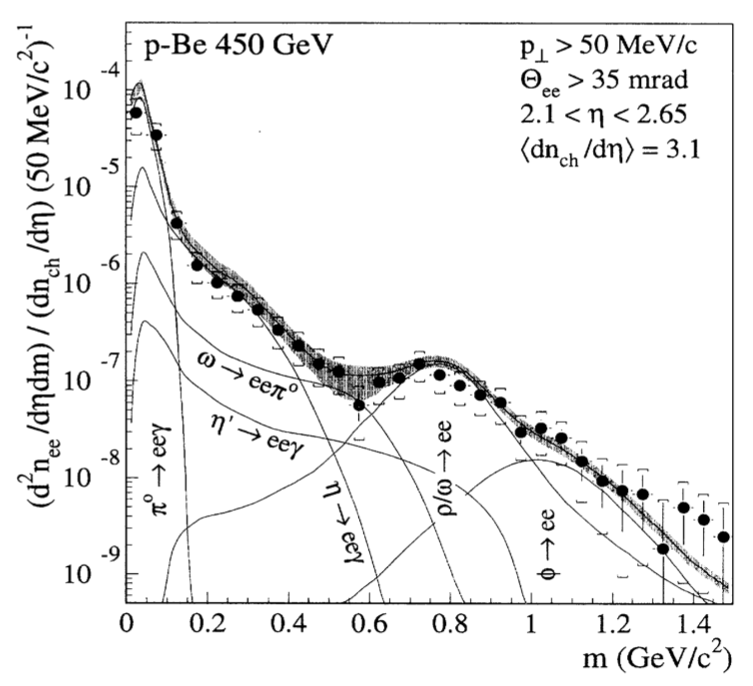
\includegraphics[width=0.33\textwidth]{fig/1.Introduction/N45_pBe}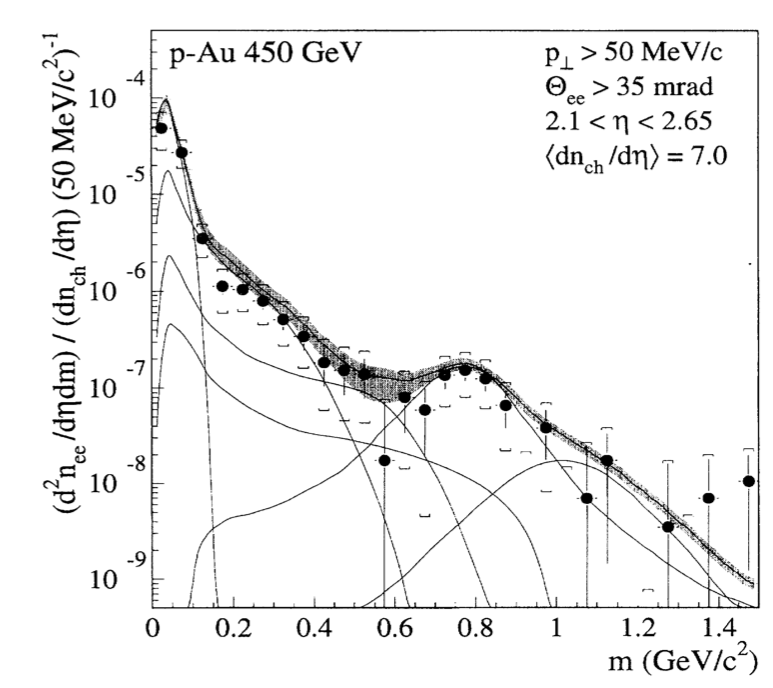
\includegraphics[width=0.33\textwidth]{fig/1.Introduction/NA45_pAu}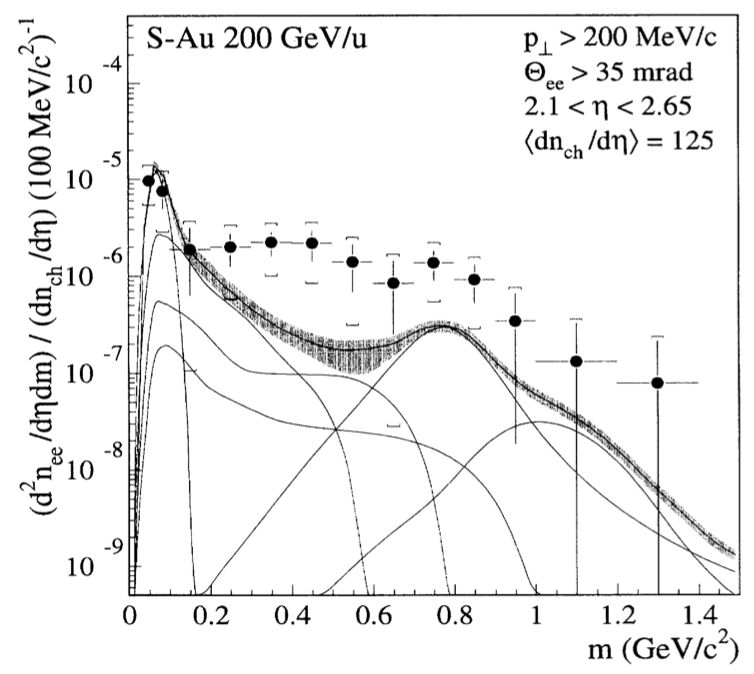
\includegraphics[width=0.33\textwidth]{fig/1.Introduction/NA45_sAu}
\par\end{centering}

\protect\caption{Inclusive $e^{+}e^{-}$ mass spectra in 450 GeV p-Be collisions (left),
p-Au collisions (middle), and 200GeV/nucleon S-Au collisions from
CERES/NA45 experiments \cite{PhysRevLett.75.1272}.}


\label{fig:NA45}
\end{figure}


\begin{figure}
\begin{centering}
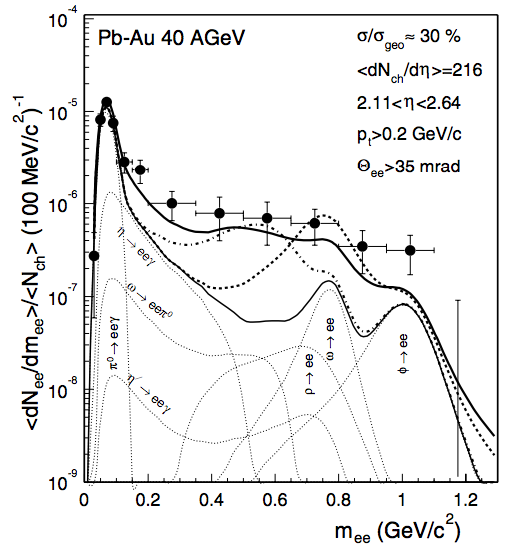
\includegraphics[width=0.8\textwidth]{fig/1.Introduction/NA45_Pb_Au_40AGeV}
\par\end{centering}

\protect\caption{Inclusive dielectron mass spectrum, compared to the hadron decay cocktail
(thin solid; individual contributions thin dotted) and to theoretical
model calculations: vacuum unmodified $\rho$ (thick dashed); in-medium
dropping $\rho$ mass (thick dash-dotted); in-medium broadening $\rho$
width ((thick solid). \cite{PhysRevLett.91.042301}}


\label{fig:NA45_Pb_Au}
\end{figure}



\subsection{NA60}

NA60 is another experiment on SPS at CERN. It inherited the muon spectrometer
and zero degree calorimeter from NA50 and equipped with a high-granularity
silicon pixel telescope vertex detector. NA60 is a muon detector and
measured the dimuon spectra which don't have large background contributed
from Dalitz decay from $\pi^{0}$. Benefited from the new vertex detectors,
NA60 can identify the offset the muon tracks with respect to the collision
vertex. The dimuon contributed from charmed meson decay thus can be
separated from prompt muon pairs.

Figure \ref{fig:NA60dimuon} left panel shows the centrality-integrated
dimuon measurement from NA60 In-In collisions at 158 AGeV. The high
data quality allows to isolate the dimuon excess from total data by
subtracting the hadronic cocktail from the known decay sources. All
hadron source except $\rho$ are included in the cocktail simulation.
The excess results are compared with the in medium modified $\rho$
model calculations. The high precision data role out the vacuum $\rho$
and dropping $\rho$ pole mass scenarios \cite{Brown200285}, and
the broadening model \cite{R.-Rapp:2000uq} can explain the data very
well. 

\begin{figure}
\begin{centering}
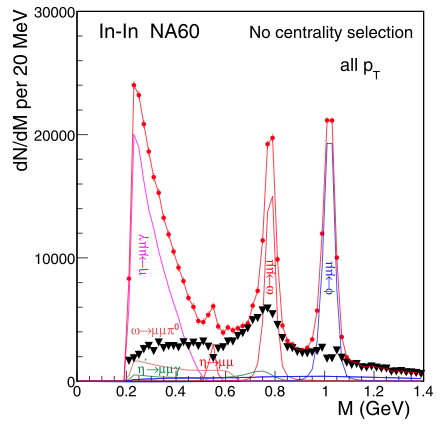
\includegraphics[width=0.45\textwidth]{fig/1.Introduction/NA60_dimuon_spec}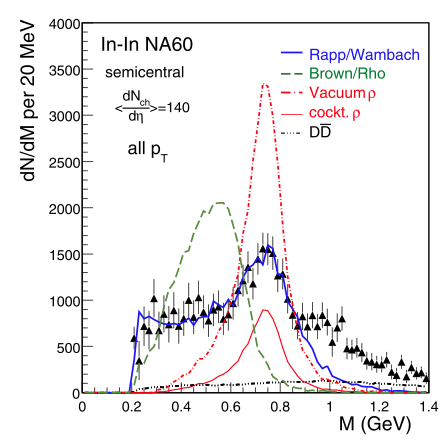
\includegraphics[width=0.45\textwidth]{fig/1.Introduction/NA60_dimuon}
\par\end{centering}

\protect\caption{(Left) Background-subtracted mass spectrum before (dots) and after
subtraction of the known decay sources (triangles). (Right) Excess
dimuons compared to theoretical predictions, renormalized to the data
in the mass interval M < 0.9 GeV. \cite{Arnaldi:2009fk}}


\label{fig:NA60dimuon}
\end{figure}


Another important results from NA60 are shown in Fig \ref{fig:NA60_Teff}.
The inverse slope parameters $T_{eff}$ of the $m_{T}$ spectra are
plotted as a function of dimuon mass in the right panel. In low mass
region ($M_{ll}<1GeV/c^{2}$), $T_{eff}$ shows a monotonic rise with
mass towards to the $\rho$ pole mass, which is a strong indication
for radial flow of a hadronic source. The measurements from hadrons
also conforms this conclusion. Around the $\phi$ mass, the $T_{eff}$
distribution shows a sudden drop about 50 MeV. This provides a first
indication of thermal leptons from a partonic source as argued by
the NA60 collaboration \cite{PhysRevLett.100.022302}. In the left
panel of Fig \ref{fig:NA60_Teff}, Acceptance-corrected invariant
mass spectrum of the excess dimuons are compared with three sets of
thermal model results \cite{PhysRevLett.100.162301,vanHees2008339,PhysRevC.80.014902},
which provide further support the conclusion of the transition from
hadronic source to partonic source from low mass to intermediate mass.
In the region above 1 GeV, all three models explicitly differentiate
between partonic and hadronic processes. In case of \cite{PhysRevLett.100.162301,PhysRevC.80.014902},
partonic source dominate and can full describe the data up to 2.5
GeV.

\begin{figure}
\begin{centering}
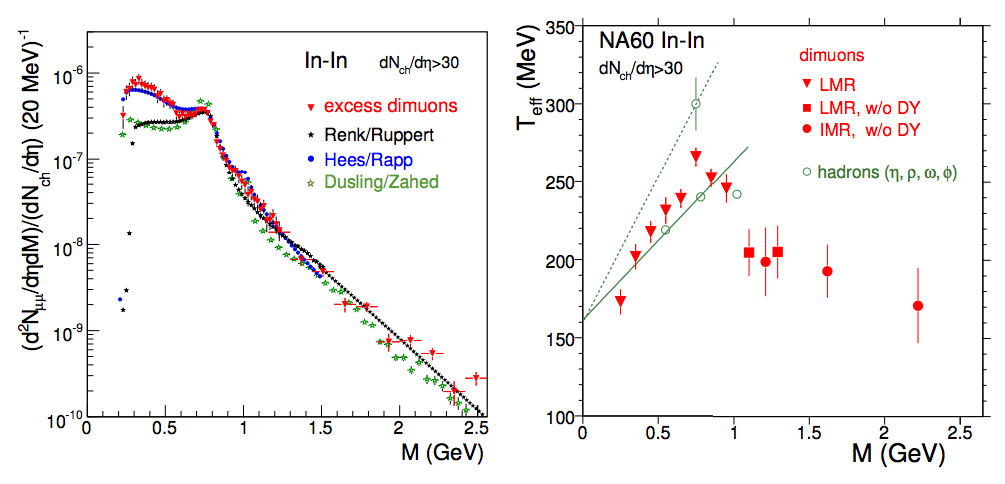
\includegraphics[width=0.9\textwidth]{fig/1.Introduction/NA60_Teff}
\par\end{centering}

\protect\caption{Left Panel: Acceptance-corrected invariant mass spectrum of the excess
dimuons, comparing with three different sets of thermal-model calculations.
Right Panel: Inverse slope parameter $T_{eff}$ of the $m_{T}$ spectra
as a function of dimuon mass. Charm contribution is removed. Hadron
results are shown for comparison. Figures are taken from \cite{NA60-Collaboration:fj}.}


\label{fig:NA60_Teff}
\end{figure}



\subsection{PHENIX}

PHENIX (Pioneering High Energy Nuclear Interaction Experiment) is
one of the two major detector system at RHIC. It is designed to mainly
study leptons and photon production from heavy ion collisions. The
PHENIX systems consists of two central arm spectrometers, each arm
covers the pseudo-rapidity range $|\eta|$ < 0.35 and an azimuthal
angle of $\pi/2$. The PHENIX collaboration reports the measurements
of inclusive mass spectrum of $e^{+}e^{-}$ pairs in p+p collision
and Au+Au collisions at $\sqrt{s}$ = 200 GeV, which are shown in
Fig \ref{fig:PHENIX_fullmass}. The $e^{+}e^{-}$ mass spectra in
p+p collision can be describe by the hadronic cocktail simulation,
while, the results from Au+Au collision shows huge enhancement in
LMR when comparing to the hadronic cocktail. The integral enhancement
observed in Au+Au collision is $4.7\pm0.4(stat.)\pm1.5(sys.)$\cite{PhysRevC.81.034911}
in mass region 0.15\textasciitilde{}0.75 GeV/$c^{2}$. The LMR excess
in 200 GeV Au+Au collisions are also compared with in-medium model
calculations in Fig \ref{fig:PHENIX_Low}, however none of them can
explain the large enhancement.

\begin{figure}
\begin{centering}
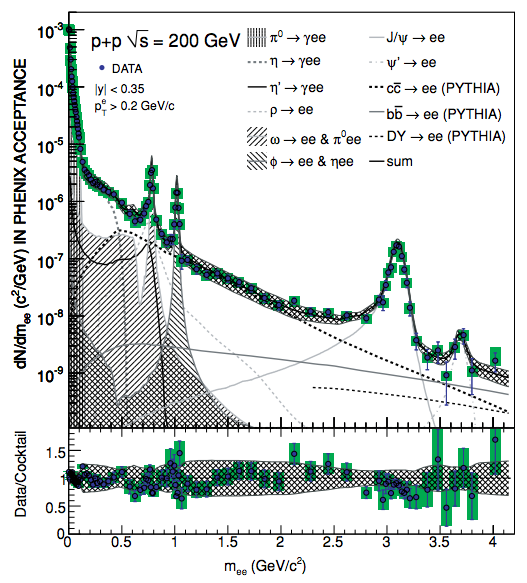
\includegraphics[width=0.45\textwidth]{fig/1.Introduction/PHENIX_PP}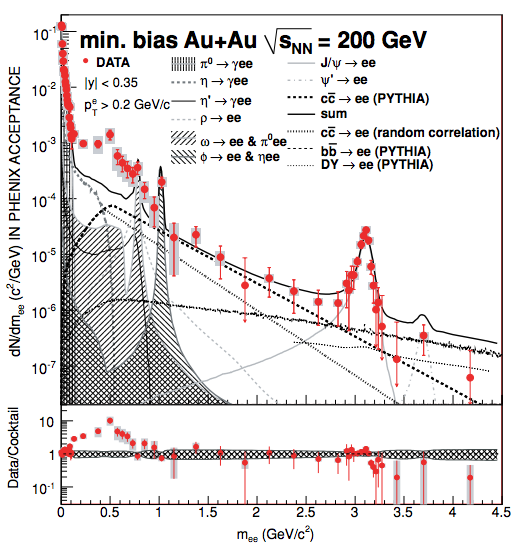
\includegraphics[width=0.45\columnwidth]{fig/1.Introduction/PHENIX_AuAu}
\par\end{centering}

\protect\caption{Inclusive mass spectrum of $e^{+}e^{-}$ pairs in the PHENIX acceptance
in minimum-bias p+p collision (left) and Au+Au collisions (right)
at $\sqrt{s}$ = 200 GeV. \cite{PhysRevC.81.034911}}


\label{fig:PHENIX_fullmass}
\end{figure}


\begin{figure}
\begin{centering}
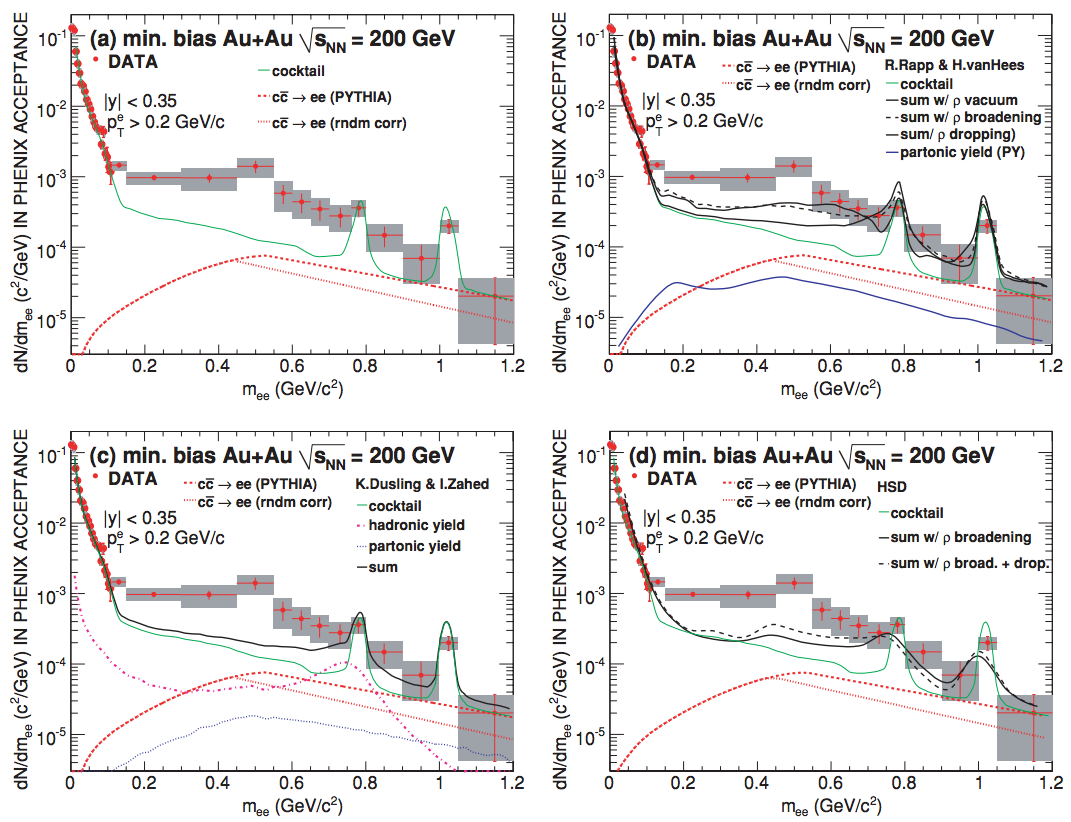
\includegraphics[width=0.8\textwidth]{fig/1.Introduction/PHENIX_LowMass}
\par\end{centering}

\protect\caption{Invariant mass spectra of e+e− pairs in Au+Au collisions in the LMR.
The data are compared to hadronic cocktail (left upper) and three
model calculations. \cite{PhysRevC.81.034911}}


\label{fig:PHENIX_Low}
\end{figure}

